\documentclass[letterpaper]{article}

% --- Packages
\usepackage[utf8]{inputenc}
\usepackage[T1]{fontenc}
\usepackage[margin=0.25cm]{geometry}
\usepackage{enumitem}
\usepackage{pdfpages}
\usepackage{multicol}
\usepackage{amsmath}
\usepackage{amssymb}
\usepackage[skip=1pt plus1pt, indent=0pt]{parskip}
\usepackage{enumitem}
\usepackage{graphicx}

% --- Data
\title{Signals and Systems 1.0}
\author{Enrique Calderon}
\date{September 2024}

% --- Graphics path
\graphicspath{ {./img/} }

% --- Custom commands
\makeatletter
\let\thetitle\@title
\let\theauthor\@author
\makeatother
\newcommand{\compconj}[1]{%
    \overline{#1}%
}
\newcommand{\divline}{\noindent\makebox[\linewidth]{\rule{\textwidth}{0.4pt}}}
\newcommand{\taninv}{\tan^{-1}}

% Example of image adding
%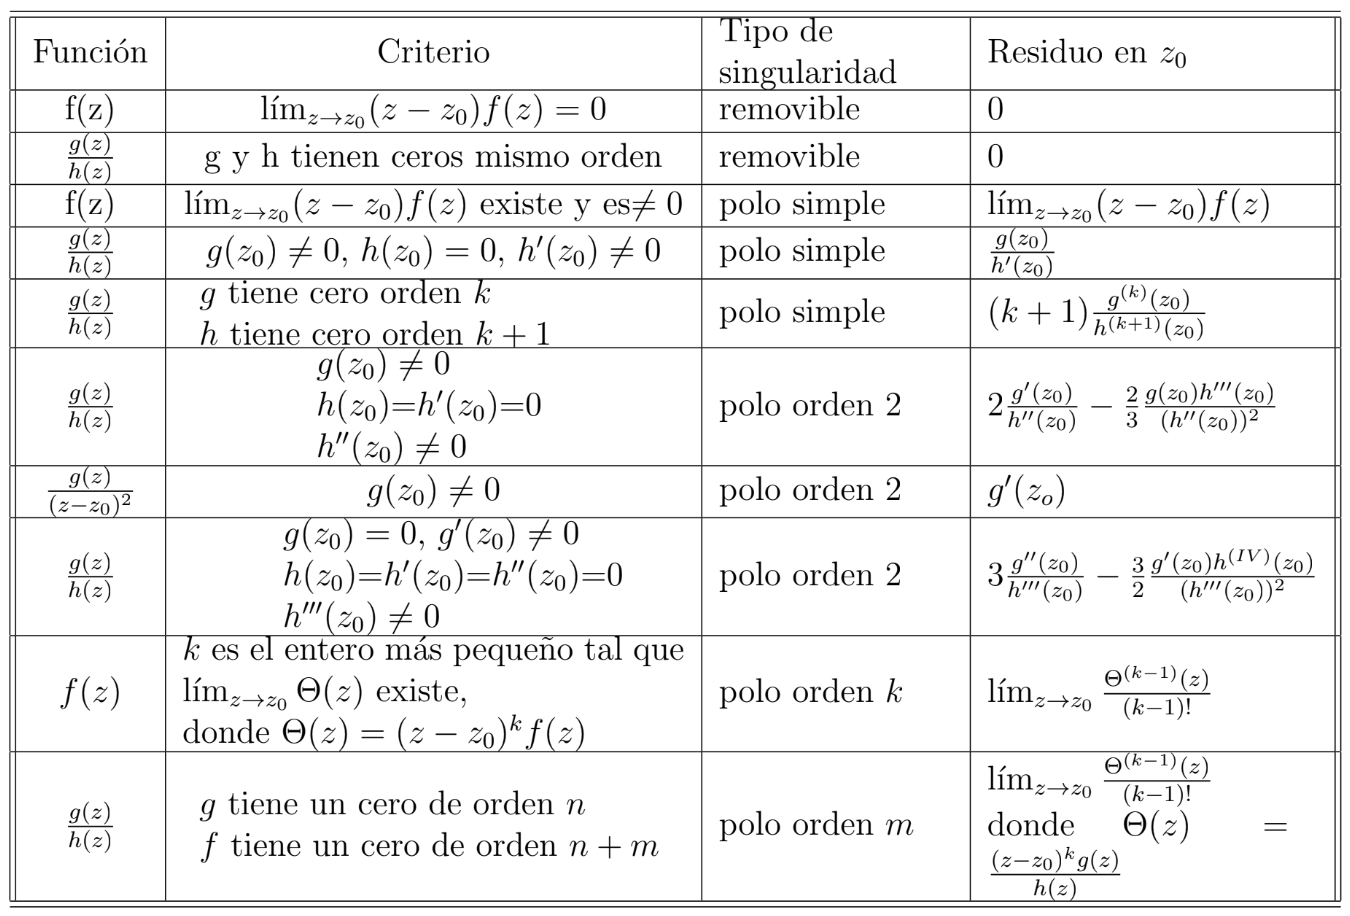
\includegraphics[width=0.8\textwidth]{ResidueTable}

% Remember to add divline between sections

\begin{document}
    \maketitle

    \divline
    \begin{multicols}{2}
        \section{Signals and Systems}

        \subsection{Periodic Signals}

        A signal $x(t)$ is periodic if there exists a positive number $T$ such that $x(t) = x(t + T)$ for all $t$.

        A signal $x[n]$ is periodic if there exists a positive number $N$ such that $x[n] = x[n + N]$ for all $n$.

        \subsection{Basic Signals in Continuous Time}

        \begin{itemize}
            \item Unit Step: $u(t) = \begin{cases} 0 & t < 0 \\ 1 & t \geq 0 \end{cases}$
            \item Unit Impulse: $\delta(t) = \begin{cases} 0 & t \neq 0 \\ \infty & t = 0 \end{cases}$
            \item Ramp: $r(t) = \begin{cases} 0 & t < 0 \\ t & t \geq 0 \end{cases}$
            \item Exponential: $e^{at}$
            \item Sinusoidal: $x(t) = A \cos{(\omega_0 t + \phi)}$ , where $\omega_0 = 2\pi f_0$ , it is periodic with fundamental period $T_0 = \frac{1}{f_0}$
            \item Complex Exponential: $e^{j\omega_0 t} = \cos{(\omega_0 t)} + j\sin{(\omega_0 t)}$ where $\omega_0 = 2\pi f_0$ is the radian frequency and $f_0$ is the frequency in Hz. It is periodic with fundamental period $T_0 = \frac{1}{f_0}$
        \end{itemize}

        \subsection{Basic Signals in Discrete Time}

        \begin{itemize}
            \item Unit Step: $u[n] = \begin{cases} 0 & n < 0 \\ 1 & n \geq 0 \end{cases}$
            \item Unit Impulse: $\delta[n] = \begin{cases} 0 & n \neq 0 \\ 1 & n = 0 \end{cases}$
            \item Ramp: $r[n] = \begin{cases} 0 & n < 0 \\ n & n \geq 0 \end{cases}$
            \item Exponential: $a^n$
            \item Sinusoidal: $x[n] = A \cos{(\Omega_0 n + \phi)}$ , where $\Omega_0 = \frac{2\pi}{N}$ , it is periodic with fundamental period $N$ when $\frac{m}{n}$ is rational.
        \end{itemize}

        \subsection{Signal Operations and Transformations}

        This operations are defined for both continuous and discrete time signals.

        \begin{itemize}
            \item Sum: $(f+g)(t) = f(t) + g(t)$
            \item Scalar Multiplication: $(\alpha f)(t) = \alpha f(t)$
            \item Linear Combination: $(\alpha f + \beta g)(t) = \alpha f(t) + \beta g(t)$
            \item Product: $(f \cdot g)(t) = f(t) \cdot g(t)$
            \item Time Shift: $(f(t-t_0))(t) = f(t-t_0)$ if $t_0 > 0$ then the signal is moved to the right, if $t_0 < 0$ then the signal is moved to the left.
            \item Inversion: $(f(-t))(t) = f(-t)$ the signal is reflected around the y-axis. If it contains a time shift, then the signal is reflected around the line $t = t_0$.
        \end{itemize}

        Just for the discrete signals we can add the following operations:

        \begin{itemize}
            \item Sum: $\sum_{n=a}^{b} x[k]= x[a] + x[a+1] + ... + x[b]$
            \item Util sum: $\sum_{n=0}^{N} b^n = \frac{1-b^{N+1}}{1-b}$
            \item Backward sum: $\Delta x[n] = \frac{\Delta x[n]}{\Delta n} = x[n] - x[n-1]$
        \end{itemize}

        \subsection{Convolution}

        The convolution integral of two signals $f(t)$ and $g(t)$ is defined as:

        \[
            (f*g)(t) = \int_{-\infty}^{\infty} f(\tau)g(t-\tau)d\tau
        \]

        The convolution sum of two signals $f[n]$ and $g[n]$ is defined as:

        \[
            (f*g)[n] = \sum_{k=-\infty}^{\infty} f[k]g[n-k]
        \]

        \subsection{Properties of Convolution}

        \begin{itemize}
            \item Commutative: $f*g = g*f$
            \item Associative: $f*(g*h) = (f*g)*h$
            \item Distributive: $f*(g+h) = f*g + f*h$
            \item Asociative with scalar: $\alpha(f) * \beta (g) = (\alpha \beta)(f*g)$
            \item Shift: $x(t) * \delta(t-t_0) = x(t-t_0)$ and $x[n] * \delta[n-n_0] = x[n-n_0]$
        \end{itemize}

        \subsection{Sampling and Reconstruction}

        Sampling is the process of converting a continuous time signal into a discrete time signal. The sampling frequency is the number of samples per second.

        \[x[n] = x_c(nT)\]

        Where $T$ is the sampling period and $F_s = \frac{1}{T}$ is the sampling frequency.

        \subsection{System Properties}

        \begin{itemize}
            \item Causality: A system is causal if the output at any time $t_0$ depends only on the input at times $t \leq t_0$.
            \item Linearity: A system is linear if it satisfies the principle of superposition. $T{\alpha x_1 + \beta x_2} = \alpha T{x_1} + \beta T{x_2}$
            \item Time Invariance: A system is time invariant if a time shift in the input signal causes a corresponding time shift in the output signal. $T{x(t)} = y(t) \Rightarrow T{x(t-t_0)} = y(t-t_0)$
            \item Stability: A system is stable if the output is bounded for any bounded input.
        \end{itemize}
    \end{multicols}

    \divline

    \begin{multicols}{2}

        \section{Linear Time-Invariant Systems}

        A system is linear if it satisfies the principle of superposition. A system is time-invariant if a time shift in the input signal causes a corresponding time shift in the output signal. A system is linear time-invariant (LTI) if it is both linear and time-invariant.

        \subsection{Impulse Response}

        The impulse response of an LTI system is the output of the system when the input is an impulse function.

        \[y(t) = x(t) * h(t)\]

        \subsection{Response}

        We can find:

        \[y = y_p + y_h\]

        Where $y_p$ is the permanent response and $y_h$ is the transient response. The first one persists while the input persists, the second one decays to zero as time goes to infinity.

        \subsection{Causality}

        A system is causal if the output at any time $t_0$ depends only on the input at times $t \leq t_0$.

        \subsection{LTI represented as EDLs}

        An LTI system can be represented as a differential equation in continuous time or as a difference equation in discrete time.

        \[\sum_{k=0}^{N} a_k \frac{d^k y(t)}{dt^k} = \sum_{k=0}^{M} b_k \frac{d^k x(t)}{dt^k}\]

        \subsection{Discrete Time FIR}

        A discrete time FIR system is a system whose output is the sum of a finite number of weighted samples of the input signal.

        \[y[n] = x[n] * h[n] = \sum_{k-\infty}^{\infty} h[k]x[n-k] = \sum_{k=0}^{L_h - 1} h[k]x[n-k]\]

        \subsection{Discrete Time IIR}

        A discrete time IIR system is a system whose output is the sum of a finite number of weighted samples of the input signal and a finite number of weighted samples of the output signal. It is recursive.

        \[y[n] = \frac{1}{a_0} \left( \sum_{k=0}^{M} b_k x[n-k] - \sum_{k=1}^{N} a_k y[n-k] \right)\]

    \end{multicols}

    \divline

    \begin{multicols}{2}
        \section{LTI System Analysis with Laplace and Z-Transforms}

        \subsection{Laplace Transform}

        The Laplace transform of a signal $x(t)$ is defined as:

        \[X(s) = \int_{0}^{\infty} x(t)e^{-st}dt\]

        The inverse Laplace transform is defined as:

        \[x(t) = \frac{1}{2\pi j} \int_{\sigma - j\infty}^{\sigma + j\infty} X(s)e^{st}ds\]

        \subsection{Properties of Laplace Transform}

        \begin{itemize}
            \item Linearity: $a_1x_1(t) + a_2x_2(t) \Leftrightarrow a_1X_1(s) + a_2X_2(s)$
            \item Convolution: $x_1(t) * x_2(t) \Leftrightarrow X_1(s)X_2(s)$
            \item Differentiation: $\frac{d^n x(t)}{dt^n} \Leftrightarrow s^nX(s) - \sum_{k=0}^{n-1} s^{n-1-k} \frac{d^k x(0)}{dt^k}$
            \item Delay in S: $e^{-at}x(t) \Leftrightarrow X(s+a)$
            \item Differentiation in S: $-tx(t) \Leftrightarrow \frac{dX(s)}{ds}$
        \end{itemize}

        \subsection{Laplace elemental transforms}

        \begin{center}
        \begin{tabular}{|c|c|}
            \hline
            $x(t)$ & $X(s)$ \\
            \hline
            $\delta(t)$ & $1$ \\
            $u(t)$ & $\frac{1}{s}$ \\
            $\frac{dx^a(t)}{dt^a}$ & $s^a X(s) - x(0) - ... - x^a(0)$ \\
            $e^{-at}u(t)$ & $\frac{1}{s+a}$ \\
            $\frac{t^{n-1}}{(n-1)!} e^{-at}u(t)$ & $\frac{1}{(s+a)^n}$ \\
            $e^{-at} \cos{(\omega_0 t)}u(t)$ & $\frac{s+a}{(s+a)^2 + \omega_0^2}$ \\
            $e^{-at} \sin{(\omega_0 t)}u(t)$ & $\frac{\omega_0}{(s+a)^2 + \omega_0^2}$ \\
            \hline
        \end{tabular}
        \end{center}

        A transformation for partial fractions is:

        \[\mathcal{L}^{-1} \left\{ \frac{Bs + C}{s^2 + \beta s + \lambda} \right\} = e^{-\alpha t} \left( A_1 \cos{(\omega_0 t)} + A_2 \sin{(\omega_0 t)} \right) u(t)\]

        Where:

        \begin{itemize}
            \item $\alpha = 0.5\beta$
            \item $\omega_0 = 0.5 \sqrt{4\lambda - \beta^2}$
            \item $A_1 = B$
            \item $A_2 = \frac{2C - \beta B}{2 \omega_0}$
        \end{itemize}

        \subsection{Transfer Function}

        The transfer function of an LTI system is the Laplace transform of the impulse response.

        \[H(s) = \frac{Y(s)}{X(s)}\]

        \subsection{Stability}

        A system is stable if all the poles of the transfer function have negative real parts.

        \subsection{Z-Transform}

        The Z-transform of a signal $x[n]$ is defined as:

        \[X(z) = \sum_{n=-\infty}^{\infty} x[n]z^{-n}\]

        For the inverse Z-transform we have:

        \[x[n] = \frac{1}{2\pi j} \oint X(z)z^{n-1}dz\]

        \subsection{Properties of Z-Transform}

        \begin{itemize}
            \item Linearity: $\alpha x_1[n] +  \beta x_2[n] \Leftrightarrow \alpha X_1(z) + \beta X_2(z)$
            \item Convolution: $x_1[n] * x_2[n] \Leftrightarrow X_1(z)X_2(z)$
            \item Time shift: $x[n-a] \Leftrightarrow z^{-a}X(z)$
            \item Scaling in Z: $a^n x[n] \Leftrightarrow X(a^{-1}z)$
            \item Differentiation in Z: $nx[n] \Leftrightarrow -z \frac{dX(z)}{dz}$
        \end{itemize}

        \subsection{Z-Transform elemental transforms}

        \begin{center}
        \begin{tabular}{|c|c|}
            \hline
            $x[n]$ & $X(z)$ \\
            \hline
            $\delta[n]$ & $1$ \\
            $u[n]$ & $\frac{z}{z - 1}$ \\
            $x[n-a]$ & $z^{-a}{X(z)}$ \\
            $a^n u[n]$ & $\frac{z}{z-a}$ \\
            $n a^n u[n]$ & $\frac{az}{(z-a)^2}$ \\
            $\rho^n \cos{(\Omega_0 n)}u[n]$ & $\frac{z^2 - z (\rho \cos{(Omega_0)} + \rho \sin{(\Omega_0)})}{z^2 - 2 \rho \cos{(\Omega_0)}z + \rho^2}$ \\
            $\rho^n \sin{(\Omega_0 n)}u[n]$ & $\frac{\rho \sin{(\Omega_0)}z}{z^2 - 2 \rho \cos{(\Omega_0)}z + \rho^2}$ \\
            \hline
        \end{tabular}
        \end{center}

        A transformation for partial fractions is:

        \[\mathcal{Z}^{-1} \left\{ \frac{Bz^2 + Cz}{z^2 + \beta z + \lambda} \right\} = \rho^n \left( A_1 \cos{(\Omega_0 n)} + A_2 \sin{(\Omega_0 n)} \right) u[n]\]

        Where:

        \begin{itemize}
            \item $\rho = \sqrt{\lambda}$
            \item $\Omega_0 = \cos^{-1}{\left( \frac{- \beta}{2 \sqrt{\lambda}} \right)}$
            \item $A_1 = B$
            \item $A_2 = \frac{2C - \beta B}{2 \rho \sin{(\Omega_0)}}$
        \end{itemize}

        \subsection{Transfer Function in Z}

        The transfer function of an LTI system is the Z-transform of the impulse response.

        \[H(z) = \frac{Y(z)}{X(z)}\]

        \subsection{Stability in Z}

        A system is stable if all the poles of the transfer function have magnitude less than 1.

        \subsection{Discretization using backwards difference}

        The backwards difference is defined as:

        \[Y'(z) = \frac{z - 1}{Tz} Y(z)\]

        \subsection{Discretization of the derivative}

        Using Barrow difference we have:

        \[Y'_c = \frac{2}{T} \left(\frac{z - 1}{z + 1}\right) Y(z)\]

        \subsection{Discretization of Systems through bilinear transformation}

        \[s = \frac{2}{T} \frac{z - 1}{z + 1}\]
    \end{multicols}

    \divline

    \begin{multicols}{2}
        \section{Miscellaneous}

        \subsection{Complex magnitude and fase}

        The magnitude of a complex number $z = a + jb$ is defined as:

        \[|z| = \sqrt{a^2 + b^2}\]

        The phase of a complex number $z = a + jb$ is defined as:

        \[\phi = \tan^{-1}{\left( \frac{y}{x} \right)}\]

        To keep it in the range $-\pi < \phi \leq \pi$ we use:

        \[\phi = \tan^{-1}{\left( \frac{y}{x} \right)} + \pi\]

        \subsection{Solve a LTI IIR system}

        To solve a LTI IIR system we can use the following steps:

        \begin{enumerate}
            \item Get $y[n] = ...$
            \item We start with $n = 0$ and we get $y[0] = ...$ substituting the values given for $x[n]$.
            \item The value $y[n-1]$ is the output of the system at time $n-1$
            \item We substitute the value of $y[n-a]$ until we get the desired $y[n]$
        \end{enumerate}

        \subsection{Solve a convolution sum}

        To solve a convolution sum we can use the following steps:

        \[x[n] * y[n]\]

        \begin{enumerate}
            \item Get $y[n] = ...$ and $x[n] = ...$
            \item Invert the signal $x[n]$ to get $x[-n]$
            \item Shift the signal $x[-n]$ to get $x[n-a]$
            \item Multiply the signals $x[n-a]y[n]$
            \item Sum the results to get the result, you will have $|x[n]| + |y[n]| - 1$ results.
        \end{enumerate}
    \end{multicols}

\end{document}
